\documentclass{article}
\usepackage{graphicx}
\usepackage[margin=1.5cm]{geometry}
\usepackage{amsmath}
\usepackage{hyperref}
\hypersetup{
    colorlinks=true,
    linkcolor=blue,
    filecolor=magenta,      
    urlcolor=cyan,
    pdftitle={Overleaf Example},
    pdfpagemode=FullScreen,
}

\begin{document}
\twocolumn

\title{Tuesday Warm Up, Unit 2: Applications}
\author{Prof. Jordan C. Hanson}
\maketitle

\section{Memory Bank}

\begin{enumerate}
\item \textbf{Short-time Fourier Transform (STFT)}.  An operation that translates a sampled, digitized signal in the time-domain, and produces amplitude versus time and frequency.
\end{enumerate}

\section{Spectrograms: the STFT}

\begin{enumerate}
\item In this exercise, we will learn to extract frequency and time information from digitized, sampled signals \\ \textit{simultaneously} using the STFT.  First, begin an \verb+octave+ script that defines a \textit{chirping} signal, similar to the final exercise of Quiz 2:
\begin{verbatim}
clear;
close;
home;

%Define a chirping signal
fs = 40.0e3; %40 kHz
dt = 1/fs;
T = 4.0; %seconds
t = dt:dt:T;
beta = 625.0; %Hz/second
f_start = 5.0e3; %1 kHz
frequencies = f_start-beta*t;
audio = 2.0*cos(2*pi*frequencies.*t);
\end{verbatim}
\item Graph \verb+audio_data+ versus time.  How is the signal changing with time?
\item The STFT algorithm in \verb+octave+ will compute the DFT of a window of the time-domain data, save the results in a column vector, and advance by a fixed increment before computing the next DFT.  The data in adjacent DFTs is smoothed when the number of DFT samples is larger than the increment.  This causes the time-slices to overlap, cancelling noise at the cost of time-resolution (\textit{think: moving average filter}).  Thus, the STFT algorithm requires the number of samples in the window function, the number of samples for the increment, and the number of DFT samples.
\item Use the following code to define the STFT of our chirping signal:
\begin{verbatim}
%Structure the spectrogram
n1 = 2048;
n2 = 128;
[sdata, info] = stft(audio,n1,n2,n1,"hamming");
sdata = sdata(1:end/2,:);
[n_freq, n_time] = size(sdata);
fbins = [0 fs/2];
tbins = [0 T];
sdata = abs(sdata);
\end{verbatim}
\item Finally, graph the \textbf{spectrogram}:
\begin{verbatim}
figure(1)
image(tbins,fbins,sdata)
xlabel('Time (seconds)')
ylabel('Frequency (Hz)')
h = colorbar();
colormap('ocean')
set(gca(),'fontsize',18)
set(h,'fontsize',18)
set(gca(),'YDir','normal');
\end{verbatim}
Do you observe the right behavior?  Why or why not?
\item Now download the \textbf{\href{https://cms.whittier.edu/mod/resource/view.php?id=683066}{LIGO Collaboration Data}} from the course Moodle page.  Use \verb+csvread()+ to load the data, and compute the STFT to reveal the chirp that served as the first evidence for graviational waves, leading to the 2017 Nobel Prize in physics.
\end{enumerate}

\begin{figure}
\centering
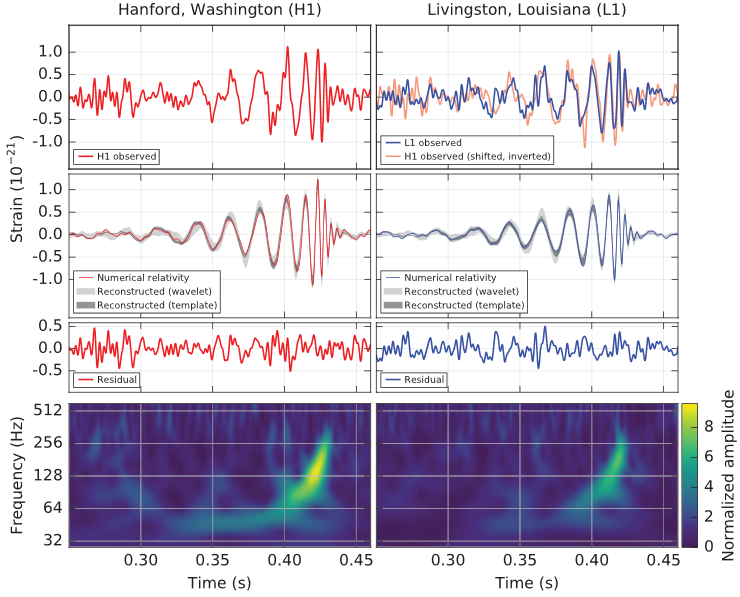
\includegraphics[width=0.45\textwidth]{LIGO_data.png}
\caption{\label{fig:1} Data corresponding to the first observations of gravitational waves, from the \textbf{\href{https://journals.aps.org/prl/abstract/10.1103/PhysRevLett.116.061102}{LIGO Collaboration}}.}
\end{figure}

\end{document}
